\section{Perceptrons multicouches}
\paragraph{}
% The first experiments I did were using images from which I extracted the eyes, as mentioned in the data processing section \ref{data-processing:eyes}.
% Each eye was resized to 60px by 30px then they were merged horizontally, forming a 120px by 30px black and white image.
% Also, each image was then labeled with a cell number, corresponding to which cell the user was looking on the given grid \ref{grid-example}.
% We will try to predict that cell number.
% Here's the first architecture that I tried:
Les premières expériences que j'ai faites ont consisté à utiliser des images dont j'ai extrait les yeux, comme mentionné dans la section \ref{data-processing:eyes} du traitement des données.
Chaque œil a été redimensionné à 60px par 30px puis ils ont été fusionnés horizontalement, formant une image noir et blanc de 120px par 30px.
De plus, chaque image a ensuite été étiquetée avec un numéro de cellule, correspondant à la cellule que l'utilisateur regardait sur la grille donnée \ref{grid-example}.
Nous allons essayer de prédire ce numéro de cellule.
Voici la première architecture que j'ai essayée :

\begin{lstlisting}[language=Python, caption=MLP 1]
model = Sequential([
    Dense(100, input_shape=(n,), kernel_initializer='glorot_uniform'),
    Dropout(0.5),
    ReLU(),
    Dense(128, kernel_initializer='glorot_uniform'),
    Dropout(0.5),
    ReLU(),
    Dense(64, kernel_initializer='glorot_uniform'),
    # Dropout(0.5),
    ReLU(),
    Dense(Config.grid_size * Config.grid_size, activation='softmax')
])
\end{lstlisting}

\paragraph{Important}
Pour les premières expériences de cette section, je n'ai utilisé que les images qui correspondaient à l'utilisateur regardant une des cellules dans les coins.
Par exemple, pour une grille de 3x3, je n'ai choisi que les images dans lesquelles l'utilisateur regardait les cellules $0, 2, 6$ ou $8$.
De plus, les données d'entraînement représentaient $80\%$ des données totales, le reste étant des données de test.

\begin{center}
    \begin{tabular}{ c | c | c | c | c | c | c }
        \hline
        Expérience & Grille taille & Taille des données & Epoques & Optimizer & Learning rate & Batch size \\ 
        \hline
        1 & 2x2 & 2184 & 300 & Adam & 0.001 & 32 \\
        \hline
        2 & 3x3 & 1247 & 300 & Adam & 0.001 & 32 \\
        \hline
        3 & 4x4 & 711 & 300 & Adam & 0.001 & 32 \\
        \hline
    \end{tabular}
\end{center}

\paragraph{}
Pour les expériences $2$ et $3$, je n'ai pris que les images correspondant aux cellules dans les coins, le nombre d'images est donc inférieur à celui de la grille 2x2.
Pour les 3 premières expériences, seule la première a bien prédit la cellule que je regardais.
Le réseau MLP s'est très bien comporté lorsque j'ai ouvert davantage les yeux, car il a mieux réussi à construire le contour de l'œil.

% For experiments 2 and 3, I only took the images corresponding to the cells in the corners, so the number of images is lower than that for the 2x2 grid.
% From the first 3 experiments, only the first predicted well at which cell I was looking.
% The MLP network did very well when I opened my eyes more, because it did a better job at building the eye contour.

\begin{figure}[H]
    \centering
    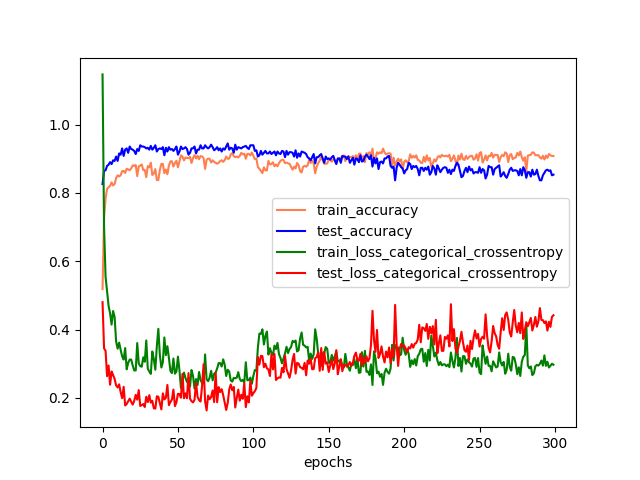
\includegraphics[width=\textwidth/3 - 5pt]{graphs/model_1.png}
    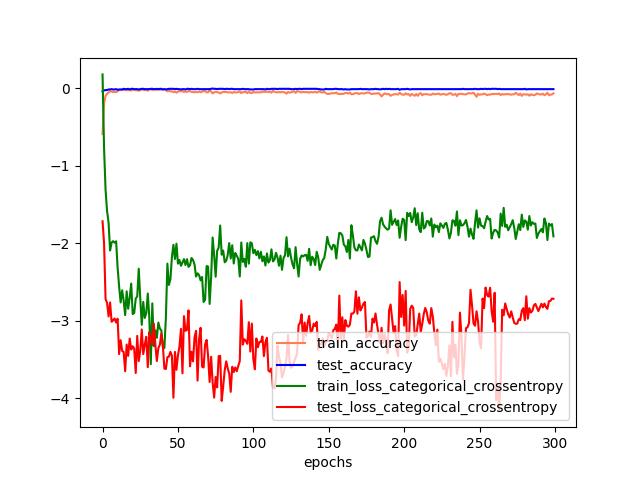
\includegraphics[width=\textwidth/3 - 5pt]{graphs/model_2.png}
    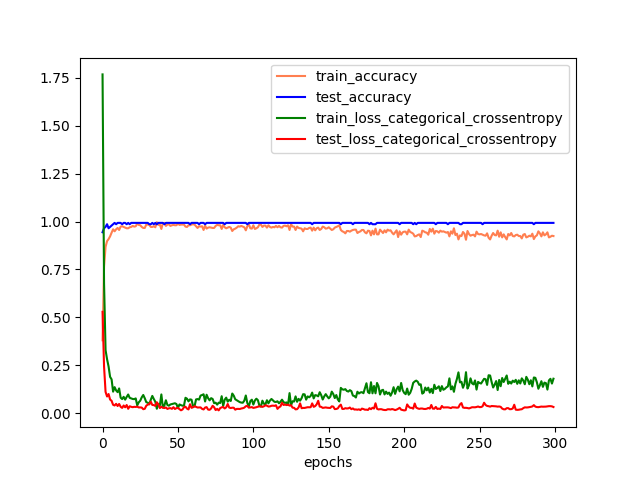
\includegraphics[width=\textwidth/3 - 5pt]{graphs/model_3.png}
    \caption{Modèles 1, 2 et 3}
\end{figure}

\paragraph{}
% We can see that the accuracies are really good for all models, but in real life the models are not that precise.
% The lighting conditions and how the user is positioned in front of the camera is very important.
Nous pouvons voir que la précision est vraiment bonne pour tous les modèles, mais dans la vie réelle, les modèles ne sont pas aussi précis.
Les conditions d'éclairage et la façon dont l'utilisateur est positionné devant la caméra sont très importantes.

\paragraph{}
Un élément important à noter, qui sera présent dans la plupart des graphiques, sont les pics, la précision allant de haut en bas.
Cela est dû à la façon dont la couche ``Dropout'' fonctionne : ``by randomly dropping units during training to prevent their co-adaptation'', comme mentionné par \cite{dropout_algorithm}.
Elle élimine les neurones aléatoires du réseau afin d'aider les autres neurones à apprendre.
Lorsqu'elle élimine les ``bons'' neurones, c'est-à-dire ceux qui donnent le plus d'informations, la précision est plus faible et l'erreur plus élevée.
Lorsqu'il élimine les neurones qui n'aident pas beaucoup à la prédiction, la précision ne sera pas trop affectée.
% An important thing to notice, that will be present in most of the graphs, are the spikes, the accuracy going up and down.
% That is caused by how the ``Dropout'' layer works.
% It eliminates random neurons from the network so it can help other neurons learn.
% When it eliminates the ``good'' neurons, that is the ones that give the most information, then the accuracy will be lower and the error higher.
% When it eliminates the neurons that don't help much in the prediction, then the accuracy will not be impacted too much.

\paragraph{}
J'ai procédé à la formation du même modèle sur la grille 3x3, mais cette fois en utilisant toutes les données dont je disposais.
Malheureusement, cela n'a pas beaucoup aidé.
J'ai également observé qu'après une certaine période, le réseau ne serait plus précis sur les données de test et qu'il serait surdimensionné.

% I proceeded in training the same model on the 3x3 grid, but this time using all the data I had.
% Unfortunately, that did not help very much.
% I also observed that after a certain epoch, the network would not be accurate on the test data and that it would overfit.

\begin{figure}[H]
    \centering
    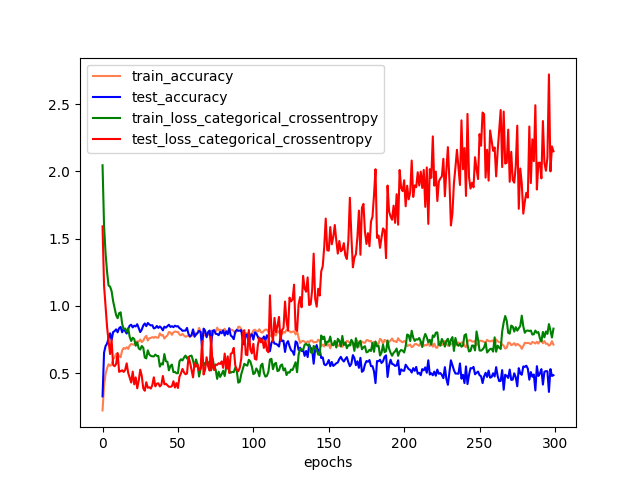
\includegraphics[width=\textwidth*2/3]{graphs/model_4.png}
    \caption{Modèle 4}
\end{figure}

\paragraph{}
Pour résoudre le problème du ``overfit'', j'ai introduit un \emph{L2 regularizer} qui, selon \cite{l1_l2_regularisation}, devrait aider à résoudre ce problème.
Cela a en effet aidé à résoudre le problème du ``overfit'', car, si l'on regarde les graphiques de précision, on peut voir que l'erreur pour les données du train est maintenant plus proche de l'erreur des données de test. Les modèles ont également mieux prédit où je regardais.

% To solve the ``overfit'' problem, I introduced an \emph{L2 regularizer} which, according to \cite{l1_l2_regularisation}, it should help with this problem.
% This indeed helped with the overfit problem and the models also did better at predicting where I was looking.

\begin{figure}[H]
    \centering
    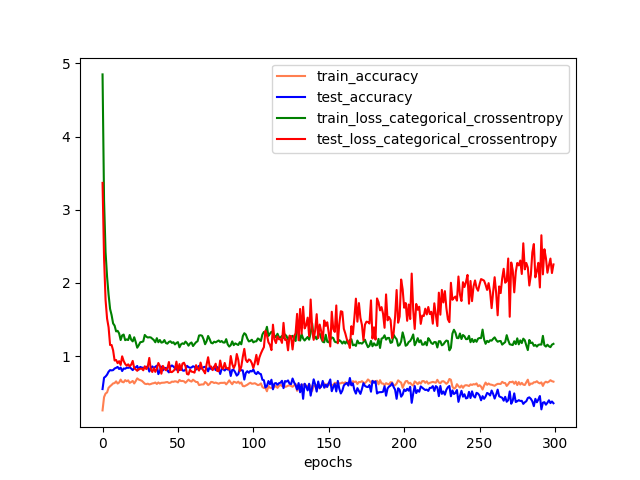
\includegraphics[width=\textwidth/2 - 5pt]{graphs/model_5.png}
    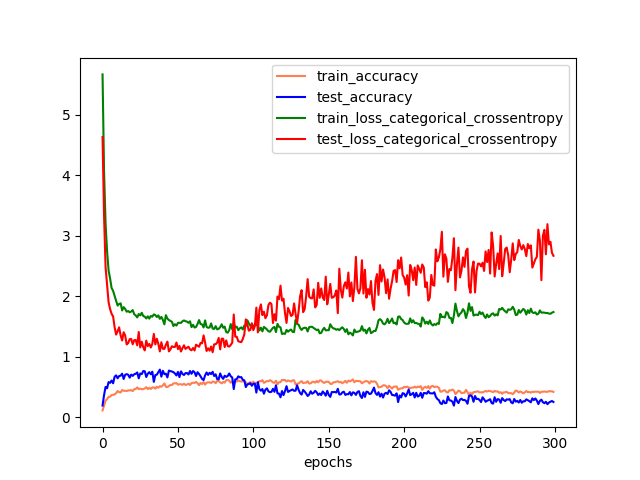
\includegraphics[width=\textwidth/2 - 5pt]{graphs/model_6.png}
    \caption{Modèles 5 et 6}
\end{figure}

% \section{Perceptrons multicouches}
% \subsection{Données utilisées}
% \paragraph{}
% Pour cette expérience, j'ai utilisé les données résultant du traitement des images originales et de l'extraction des seuls yeux \ref{data-processing:eyes}.
% Le nombre de cas était $\approx500$, les résultats pourraient donc ne pas être très précis.
% Je vais relancer cette expérience avec plus de données.
% % For this experiment, I used the data resulted from processing the original images and extracting only the eyes \ref{data-processing:eyes}.
% % The number of instances was $\approx500$, so the results might not be very accurate.
% % I will rerun this experiment with more data.

% \subsection{Paramètres d'entraînement}
% \paragraph{}
% J'ai entraîné ce modèle en utilisant la configuration ci-dessous, pour environ 1000 époques.
% J'ai essayé plusieurs optimiseurs, tels que Adam, Adagrad et SGD, mais RMSprop semblait faire les choses très bien.
% % I trained this model using the configuration below, for about 1000 epochs.
% % I tried multiple optimizers, such as Adam, Adagrad and SGD, but RMSprop seemed to do things just fine.

% \begin{lstlisting}[language=python, caption=Formation du MLP]
% print('Loading train data...')
% X, y = get_data()
% X = np.array(X)
% y = np.array(y)

% print('Training neural network...')
% model = Sequential([
%     Dense(100, input_shape=(len(X[0]),),
%             kernel_initializer='glorot_uniform'),
%     Dropout(0.5),
%     ReLU(),
%     Dense(16, kernel_initializer='glorot_uniform'),
%     ReLU(),
%     Dense(4, activation='softmax')
% ])
% rmsprop = RMSprop(lr=0.001)
% model.compile(optimizer='adagrad',
%                 loss='categorical_crossentropy', metrics=['accuracy'])
% start_time = time.time()
% fit_history = model.fit(X, y, epochs=train_parameters["epochs"], verbose=1)
% end_time = time.time()
% print('Training done')
% \end{lstlisting}

% \subsection{Résultats}
% \paragraph{}
% Les tests effectués sur les mêmes données de formation ont donné une précision de plus de $95\%$.
% Je vais réexaminer le score des mesures sur des données de test distinctes, après en avoir acquis d'autres.
% Cependant, j'ai essayé de prédire où l'utilisateur regarde sur une grille de 2x2 et cela a donné de bons résultats dans l'ensemble.
% Bien que ce ne soit pas parfait, il a fait le travail.
% % Testing this on the same training data gave an accuracy of over $95\%$.
% % I will rerun the metrics score on some separate testing data, after I will have acquired more.
% % However, I tried predicting where the user is looking on a 2x2 grid and it did mostly well.
% % While it wasn't perfect, it did the job.

% \begin{figure}[h]
%     \centering
%     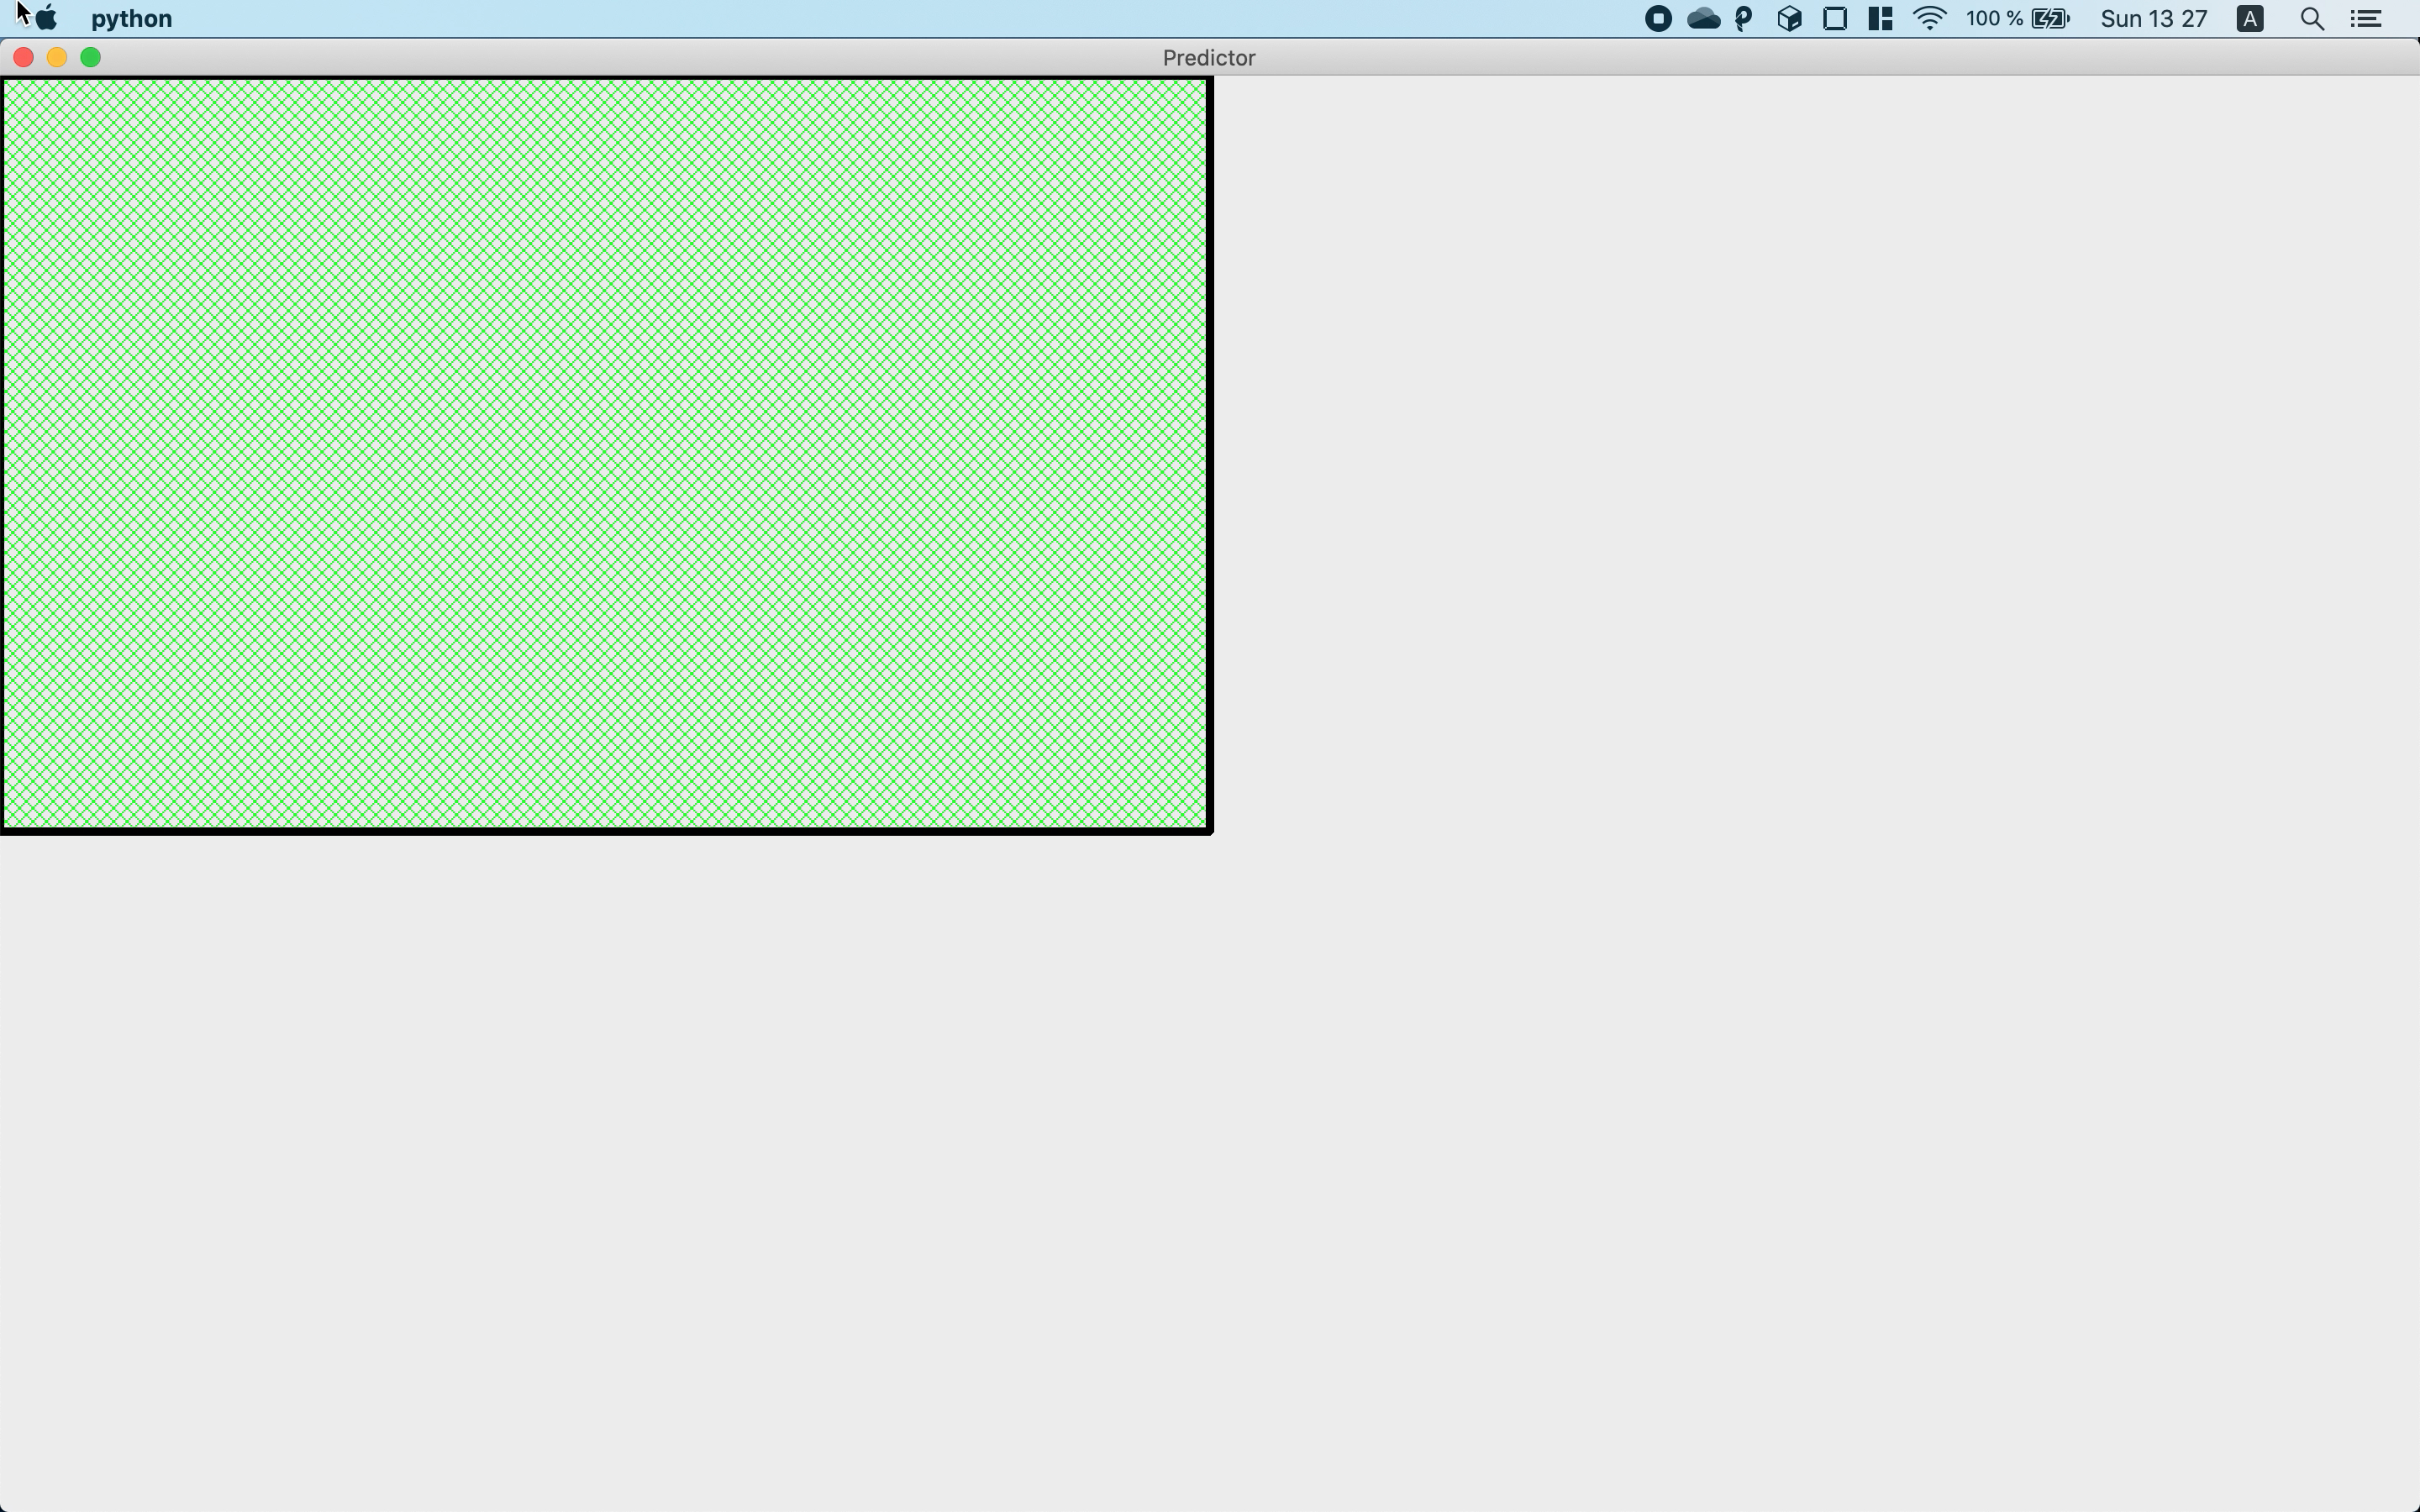
\includegraphics[width=\textwidth]{mlp_prediction.png}
%     \caption{Prévision sur une grille 2x2 avec MLP\\En fait, je vraiment regardais dans la partie supérieure gauche de l'écran, croyez-moi!}
%     \label{}
% \end{figure}

\section{Réseaux neuronaux convolutifs}
\subsection{Utilisation des visages extraits comme données}
\paragraph{}
La première expérience que j'ai faite consistait à utiliser les visages extraits \ref{fig_extracted_faces} sur une grille de 2x2 \ref{grid-example}.
Malheureusement, ce fut un échec.
Après avoir analysé le code, j'ai découvert que j'avais un bug et que les données n'étaient pas normalisées, ce qui empêchait la CNN d'apprendre.
J'ai résolu ce problème et j'ai commencé à expérimenter.

\paragraph{}
Voici l'architecture réseau que j'ai utilisée :

\label{cnn_first_architecture}
\begin{lstlisting}[language=Python, caption=Première architecture de CNN]
model = Sequential()
model.add(Conv2D(16, kernel_size=(3, 3),
                    input_shape=input_shape))
model.add(MaxPooling2D(pool_size=(2, 2)))
model.add(ReLU())
model.add(Conv2D(32, kernel_size=(3, 3)))
model.add(MaxPooling2D(pool_size=(2, 2)))
model.add(ReLU())
model.add(Flatten())
model.add(Dense(128, activation='relu'))
model.add(Dense(4, activation='softmax'))
# optimizer used
opt = Adam()
\end{lstlisting}

\paragraph{Important}
Pour les premières expériences de cette section, je n'ai utilisé que les images qui correspondaient à l'utilisateur regardant une des cellules dans les coins.Par exemple, pour une grille de 3x3, je n'ai choisi que les images dans lesquelles l'utilisateur regardait les cellules $0, 2, 6$ ou $8$.
De plus, les données d'entraînement représentaient $80\%$ des données totales, le reste étant des données de test.

% For the following experiments, I only used the data that was close to the corners.
% For example, for a grid of 3x3, I only chose the images in which the user was looking at cells $0, 2, 6$ or $8$.
% Also, the training data consisted in $80\%$ of the total data, and the rest of it was testing data.

\paragraph{}
Voici les paramètres :

\begin{center}
    \begin{tabular}{ c | c | c | c | c | c | c }
        \hline
        Expérience & Grille taille & Taille des données & Epoques & Optimizer & Learning rate & Batch size \\ 
        \hline
        7 & 2x2 & 2184 & 50 & Adam & 0.001 & 32 \\
        \hline
        8 & 3x3 & 1247 & 50 & Adam & 0.001 & 32 \\
        \hline
        9 & 4x4 & 711 & 50 & Adam & 0.001 & 32 \\
        \hline
    \end{tabular}
\end{center}

\paragraph{}
% Here we can see how the models perform:
Ici, nous pouvons voir comment les modèles se comportent :

\begin{figure}[H]
    \centering
    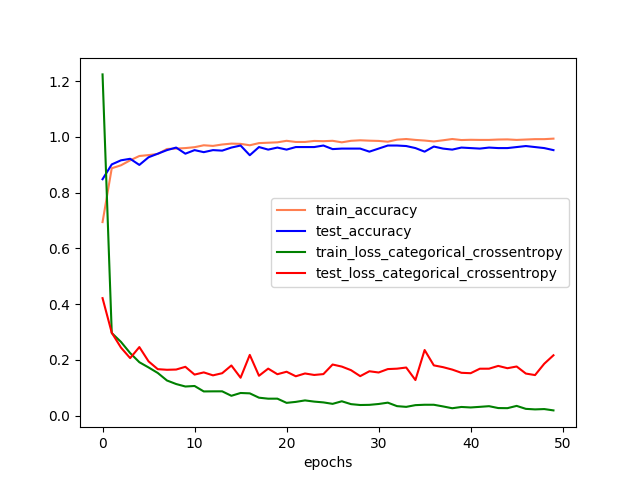
\includegraphics[width=\textwidth/3 - 5pt]{graphs/model_7.png}
    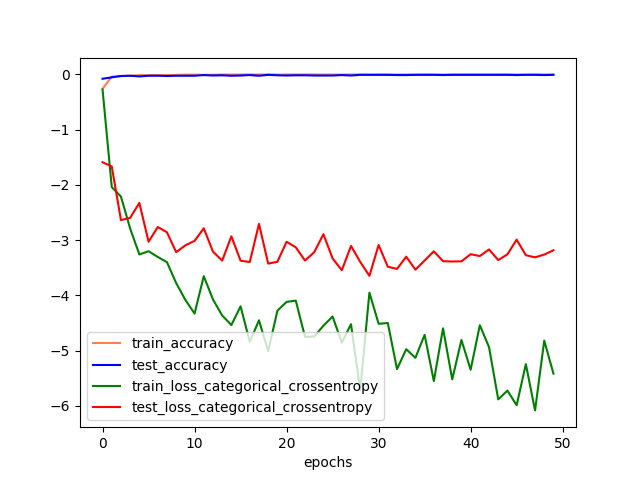
\includegraphics[width=\textwidth/3 - 5pt]{graphs/model_8.png}
    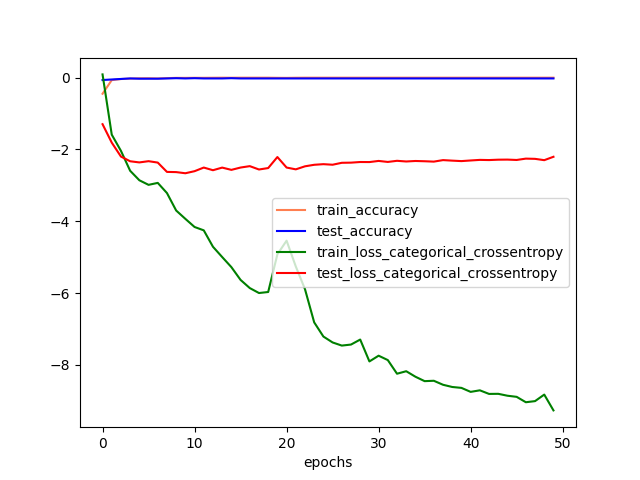
\includegraphics[width=\textwidth/3 - 5pt]{graphs/model_9.png}
    \caption{Modèles 7, 8 et 9}
\end{figure}

\paragraph{}
Les modèles $8$ et $9$ ont eu de bons scores, mais ils étaient instables quand il s'agissait de prédire où je regardais.
Le modèle $7$ a fait mieux : si je m'assieds dans le bon angle, il peut prédire assez bien où je regarde.
Cela est probablement dû au fait que le modèle a été entraîné avec plus de données.

% Models $8$ and $9$ had good scores, but they were unstable when predicting where I was looking.
% Model $7$ did better: if I sit at the right angle, it can predict fairly well where I'm looking.
% This is probably because the model was trained with more data.

\paragraph{}
Pour les expériences $10$ et $11$, j'ai rassemblé plus d'images et j'ai formé la même CNN sur l'ensemble des données (pas seulement les données de coin), ce qui représente environ $2736$ d'images, pour des grilles de 3x3 et 4x4.
Les prévisions avec ces modèles étaient meilleures, ce qui m'a poussé à la conclusion que plus j'avais de données, mieux c'était.
On peut également voir un signe de "surcharge" dans ces modèles.

% For experiments $10$ and $11$, I gathered more images and trained the same CNN on the whole data (not just corner data), which is about $2736$ images, for grid sizes of 3x3 and 4x4.
% Predicting with these models was better, which lead me to the conclusion that the more data I have, the better.
% We can also see a sign of ``overfit'' in these models.

\begin{figure}[H]
    \centering
    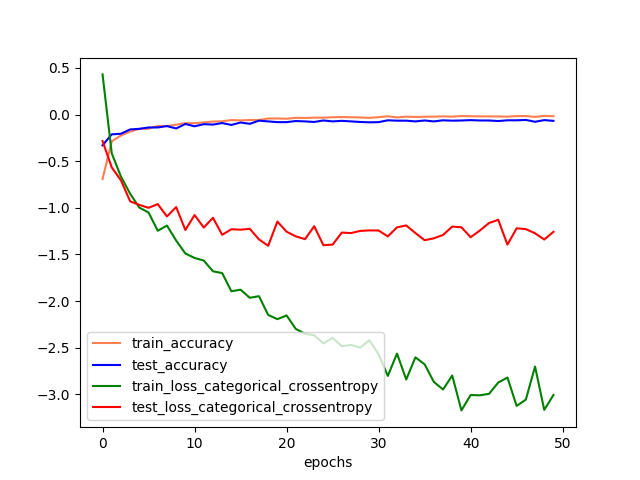
\includegraphics[width=\textwidth/2 - 5pt]{graphs/model_10.png}
    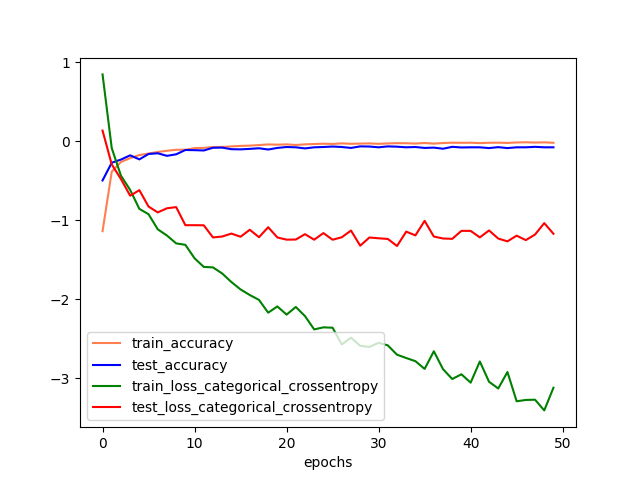
\includegraphics[width=\textwidth/2 - 5pt]{graphs/model_11.png}
    \caption{Modèles 10 et 11}
\end{figure}

\subsection{Utilisation de ``bandes oculaire'' comme données}
\paragraph{}
J'ai utilisé la même architecture CNN que celle ci-dessus, mais cette fois en utilisant des données différentes \ref{fig_extracting_eye_strip}.
Les premières expériences n'utilisaient que des images dans lesquelles l'utilisateur regardait près des coins de l'écran.
% I used the same CNN architecture as the one above, but this time using different data \ref{fig_extracting_eye_strip}.
% The first experiments were using only images in which the user was looking close to the corners of the screen.

\begin{center}
    \begin{tabular}{ c | c | c | c | c | c | c }
        \hline
        Expérience & Grille taille & Taille des données & Epoques & Optimizer & Learning rate & Batch size \\ 
        \hline
        12 & 2x2 & 2184 & 50 & Adam & 0.001 & 32 \\
        \hline
        13 & 3x3 & 1247 & 50 & Adam & 0.001 & 32 \\
        \hline
        14 & 4x4 & 711 & 50 & Adam & 0.001 & 32 \\
        \hline
    \end{tabular}
\end{center}

\begin{figure}[H]
    \centering
    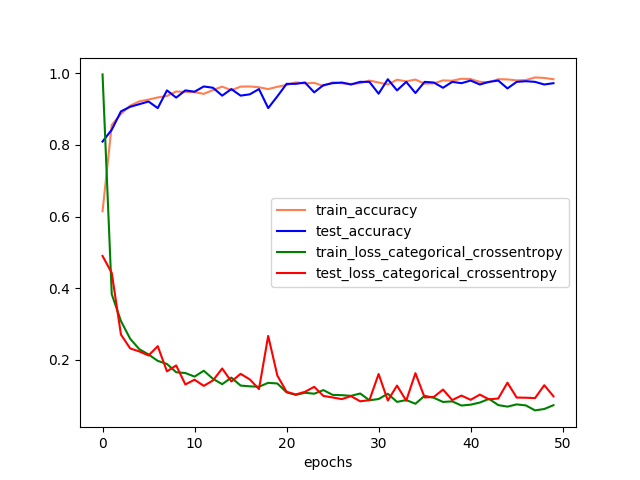
\includegraphics[width=\textwidth/3 - 5pt]{graphs/model_12.png}
    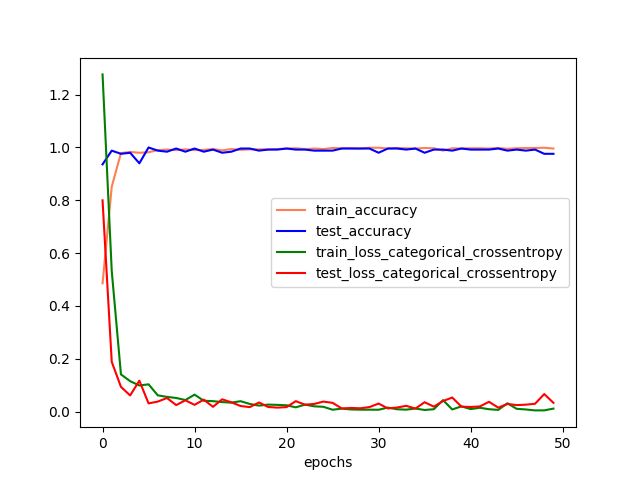
\includegraphics[width=\textwidth/3 - 5pt]{graphs/model_13.png}
    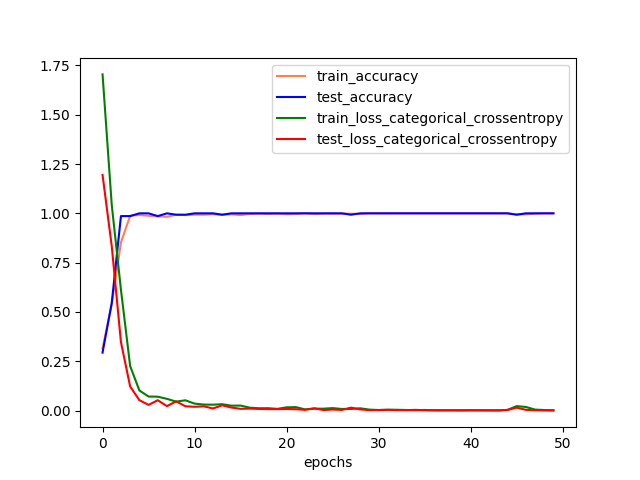
\includegraphics[width=\textwidth/3 - 5pt]{graphs/model_14.png}
    \caption{Modèles 12, 13 et 14}
\end{figure}

\paragraph{}
L'expérience $12$ était bonne, meilleure que la plupart des autres jusqu'à présent.
Elle pouvait assez bien prédire où je regardais, même si je m'éloignais de l'écran.
Les expériences $13$ et $14$ n'étaient pas si bonnes, même si elles avaient une bonne précision et de faibles erreurs.
Une fois de plus, cela s'est probablement produit parce que le modèle formé sur une grille 2x2 obtient plus de données, car pour ces expériences, j'ai seulement sélectionné les images dans lesquelles l'utilisateur regarde une cellule de coin, et sur une grille 2x2, chaque image correspond à un coin.
% Experiment 12 was great.
% It could predict fairly well where I was looking, even if I was distancing myself from the screen.
% Experiments 13 and 14 weren't so good, even though they had good accuracies and low losses.
% This, once again, probably happened because the model trained on a 2x2 grid gets more data, because for these experiments I only selected the images in which the user looks at a corner cell, and on a 2x2 grid each image corresponds to a corner.

\paragraph{}
Pour les expériences $15$ et $16$, j'ai entraîné la même CNN sur des grilles de 3x3 et 4x4, mais cette fois en utilisant toutes les données dont je dispose.
Cette fois, ils ont fait de meilleures prévisions, surtout quand je regardais dans les coins.
Cependant, avec les modèles $15$ et $16$, lorsque je regardais au centre de l'écran, on disait parfois que je regardais l'un des coins.

% For experiments 15 and 16, I trained the same CNN on grid sizes of 3x3 and 4x4, but this time using all of the data that I have.
% This time, they were predicting better, especially when I was looking in the corners.
% However, with models 15 and 16, when I was looking in the center of the screen, it would sometimes say I was looking at one of the corners.

\begin{figure}[H]
    \centering
    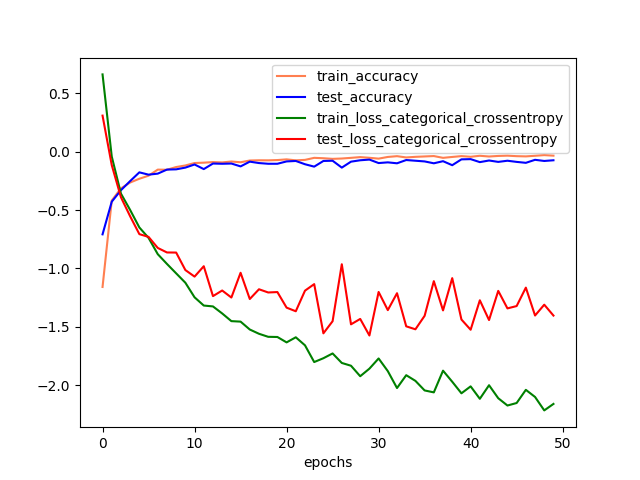
\includegraphics[width=\textwidth/2 - 5pt]{graphs/model_15.png}
    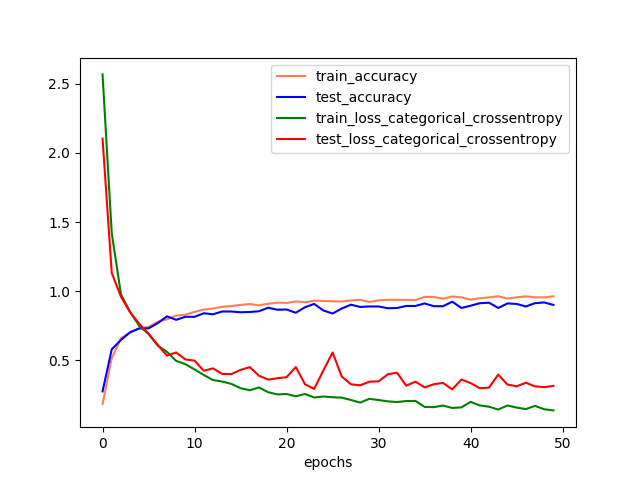
\includegraphics[width=\textwidth/2 - 5pt]{graphs/model_16.png}
    \caption{Modèles 15 et 16}
\end{figure}

\paragraph{Commentaire jusqu'à présent}
D'après les expériences menées jusqu'à présent, j'ai conclu que CNN en combinaison avec des ``bandeau oculaire'' est la meilleure option.
De plus, lorsque j'ai entraîné le même modèle sur un plus grand nombre de données, il a toujours donné de meilleurs résultats.
Il est donc extrêmement important d'avoir le plus de données possible et aussi une certaine variété dans les images que j'utilise.
% From the experiments so far, I concluded that CNN in combination with ``eye strips'' is the best option.
% Also, when I trained the same model on more data, it always did better, so it is extremely important to have as much data as possible and also have some variety in the images I use.

\subsection{Améliorer l'architecture de CNN}
\paragraph{}
Les expériences $17-22$ consistaient à essayer d'améliorer la première architecture de CNN \ref{cnn_first_architecture}.
J'ai essayé de supprimer une des couches de convolution et de modifier le nombre de filtres de convolution.

% Experiments 17-22 consisted in trying to improve the first CNN architecture \ref{cnn_first_architecture}.
% I tried removing one of the convolution layers and changing the number of convolution filters.

\paragraph{}
J'ai remarqué que lorsque j'ai retiré la deuxième couche de convolution, le réseau ne pouvait pas prédire certaines cellules qu'il avait correctement prédites auparavant (par exemple la cellule numéro $2$ sur une grille 3x3).
De plus, en augmentant le nombre de filtres de convolution, les prédictions s'amélioraient, j'ai donc décidé de continuer avec cette architecture :
% I noticed that when I removed the second layer of convolution, the network couldn't predict some cells that it correctly predicted before (for example cell number 2 on a 3x3 grid).
% Also, when increasing the number of convolution filters, the predictions would improve, so I decided to continue with this architecture:

\begin{lstlisting}[language=Python, caption=Nouvelle architecture de la cnn]
model = Sequential()
model.add(Conv2D(64, kernel_size=(3, 3),
                    input_shape=input_shape))
model.add(MaxPooling2D(pool_size=(2, 2)))
model.add(ReLU())
model.add(Conv2D(128, kernel_size=(3, 3)))
model.add(MaxPooling2D(pool_size=(2, 2)))
model.add(ReLU())
model.add(Flatten())
model.add(Dense(128, activation='relu'))
model.add(Dense(Config.grid_size * Config.grid_size, activation='softmax'))
\end{lstlisting}

\section{Régression avec CNN}
\paragraph{}
% For my next experiments, I tried to predict the exact mouse position, and based on that, see what cell the user is looking at.
Pour mes prochaines expériences, j'ai essayé de prédire la position exacte de la souris et, sur cette base, de voir quelle cellule l'utilisateur regarde.
\begin{center}
    \begin{tabular}{ c | c | c | c | c | c | c }
        \hline
        Expérience & Grille taille & Taille des données & Epoques & Optimizer & Learning rate & Batch size \\ 
        \hline
        22 & 3x3 & 2736 & 50 & Adam & 0.001 & 32 \\
        \hline
        23 & 3x3 & 2736 & 100 & \vtop{\hbox{\strut Adam}\hbox{\strut decay=$10^{-4}$}} & 0.001 & 32 \\
        \hline
        24 & 3x3 & 2736 & 100 & \vtop{\hbox{\strut Adam}\hbox{\strut decay=$10^{-4}$}} & 0.01 & 32 \\
        \hline
    \end{tabular}
\end{center}

\paragraph{}
Au début, l'expérience $22$ était chaotique, mais j'ai découvert que si je tiens l'ordinateur portable dans le bon angle et à la bonne hauteur, les prédictions sont assez bonnes.
Par la suite, j'ai formé le même modèle pour d'autres époques et j'ai également introduit une diminution du taux d'apprentissage, qui actualise le taux d'apprentissage par cette formule :
\lstinline{lr = initial_lr * (1 / (1 + decay * iteration))}.
Cela a permis au réseau d'apprendre rapidement au début, puis d'apprendre plus lentement, mais de s'améliorer encore à la fin.
Ces modèles étaient les meilleurs jusqu'à présent.
% At first, experiment 22 was chaotic, but I found that if I hold the laptop at the right angle and at the right height, the predictions are quite good.
% Afterwards, I trained the same model for more epochs and I also introduced a ``learning rate decay'', which updates the learning rate by this formula:
% \lstinline{lr = initial_lr * (1 / (1 + decay * iteration))}.
% This allowed the network to learn fast at the beggining, and then learn slower, but still improve in the latter epochs
% These models were the best so far.

\begin{figure}[H]
    \centering
    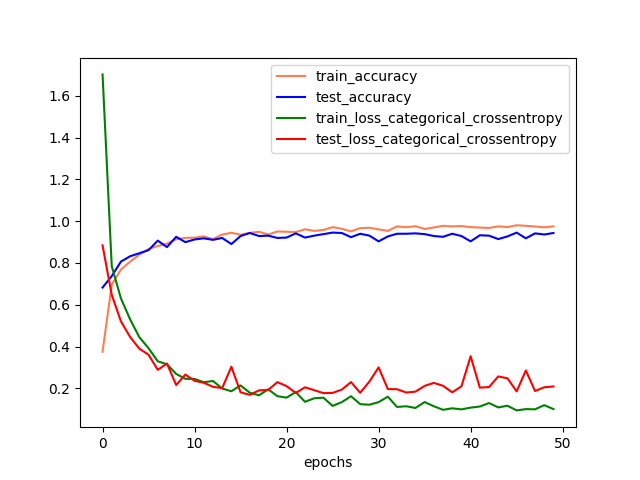
\includegraphics[width=\textwidth/3 - 5pt]{graphs/model_22.png}
    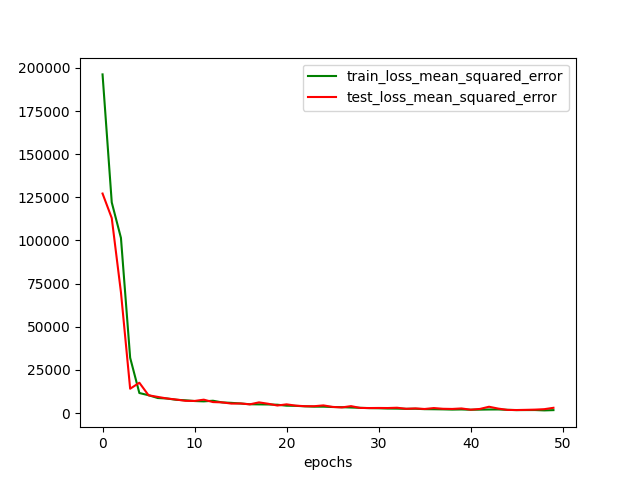
\includegraphics[width=\textwidth/3 - 5pt]{graphs/model_23.png}
    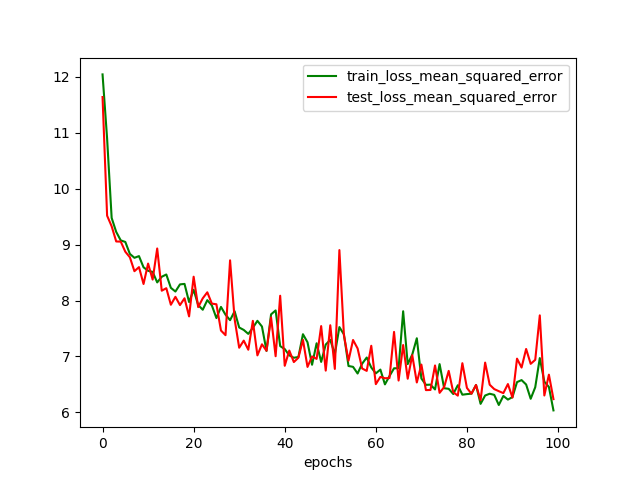
\includegraphics[width=\textwidth/3 - 5pt]{graphs/model_24.png}
    \caption{Modèles 12, 13 et 14}
\end{figure}

\section{Comment sont extraits les repères faciaux}
\paragraph{}
Après avoir utilisé avec succès l'architecture CNN pour prédire la zone où l'utilisateur regarde, je me suis intéressé à la manière dont les points de repère faciaux peuvent être détectés.

\begin{figure}[h]
    \centering
    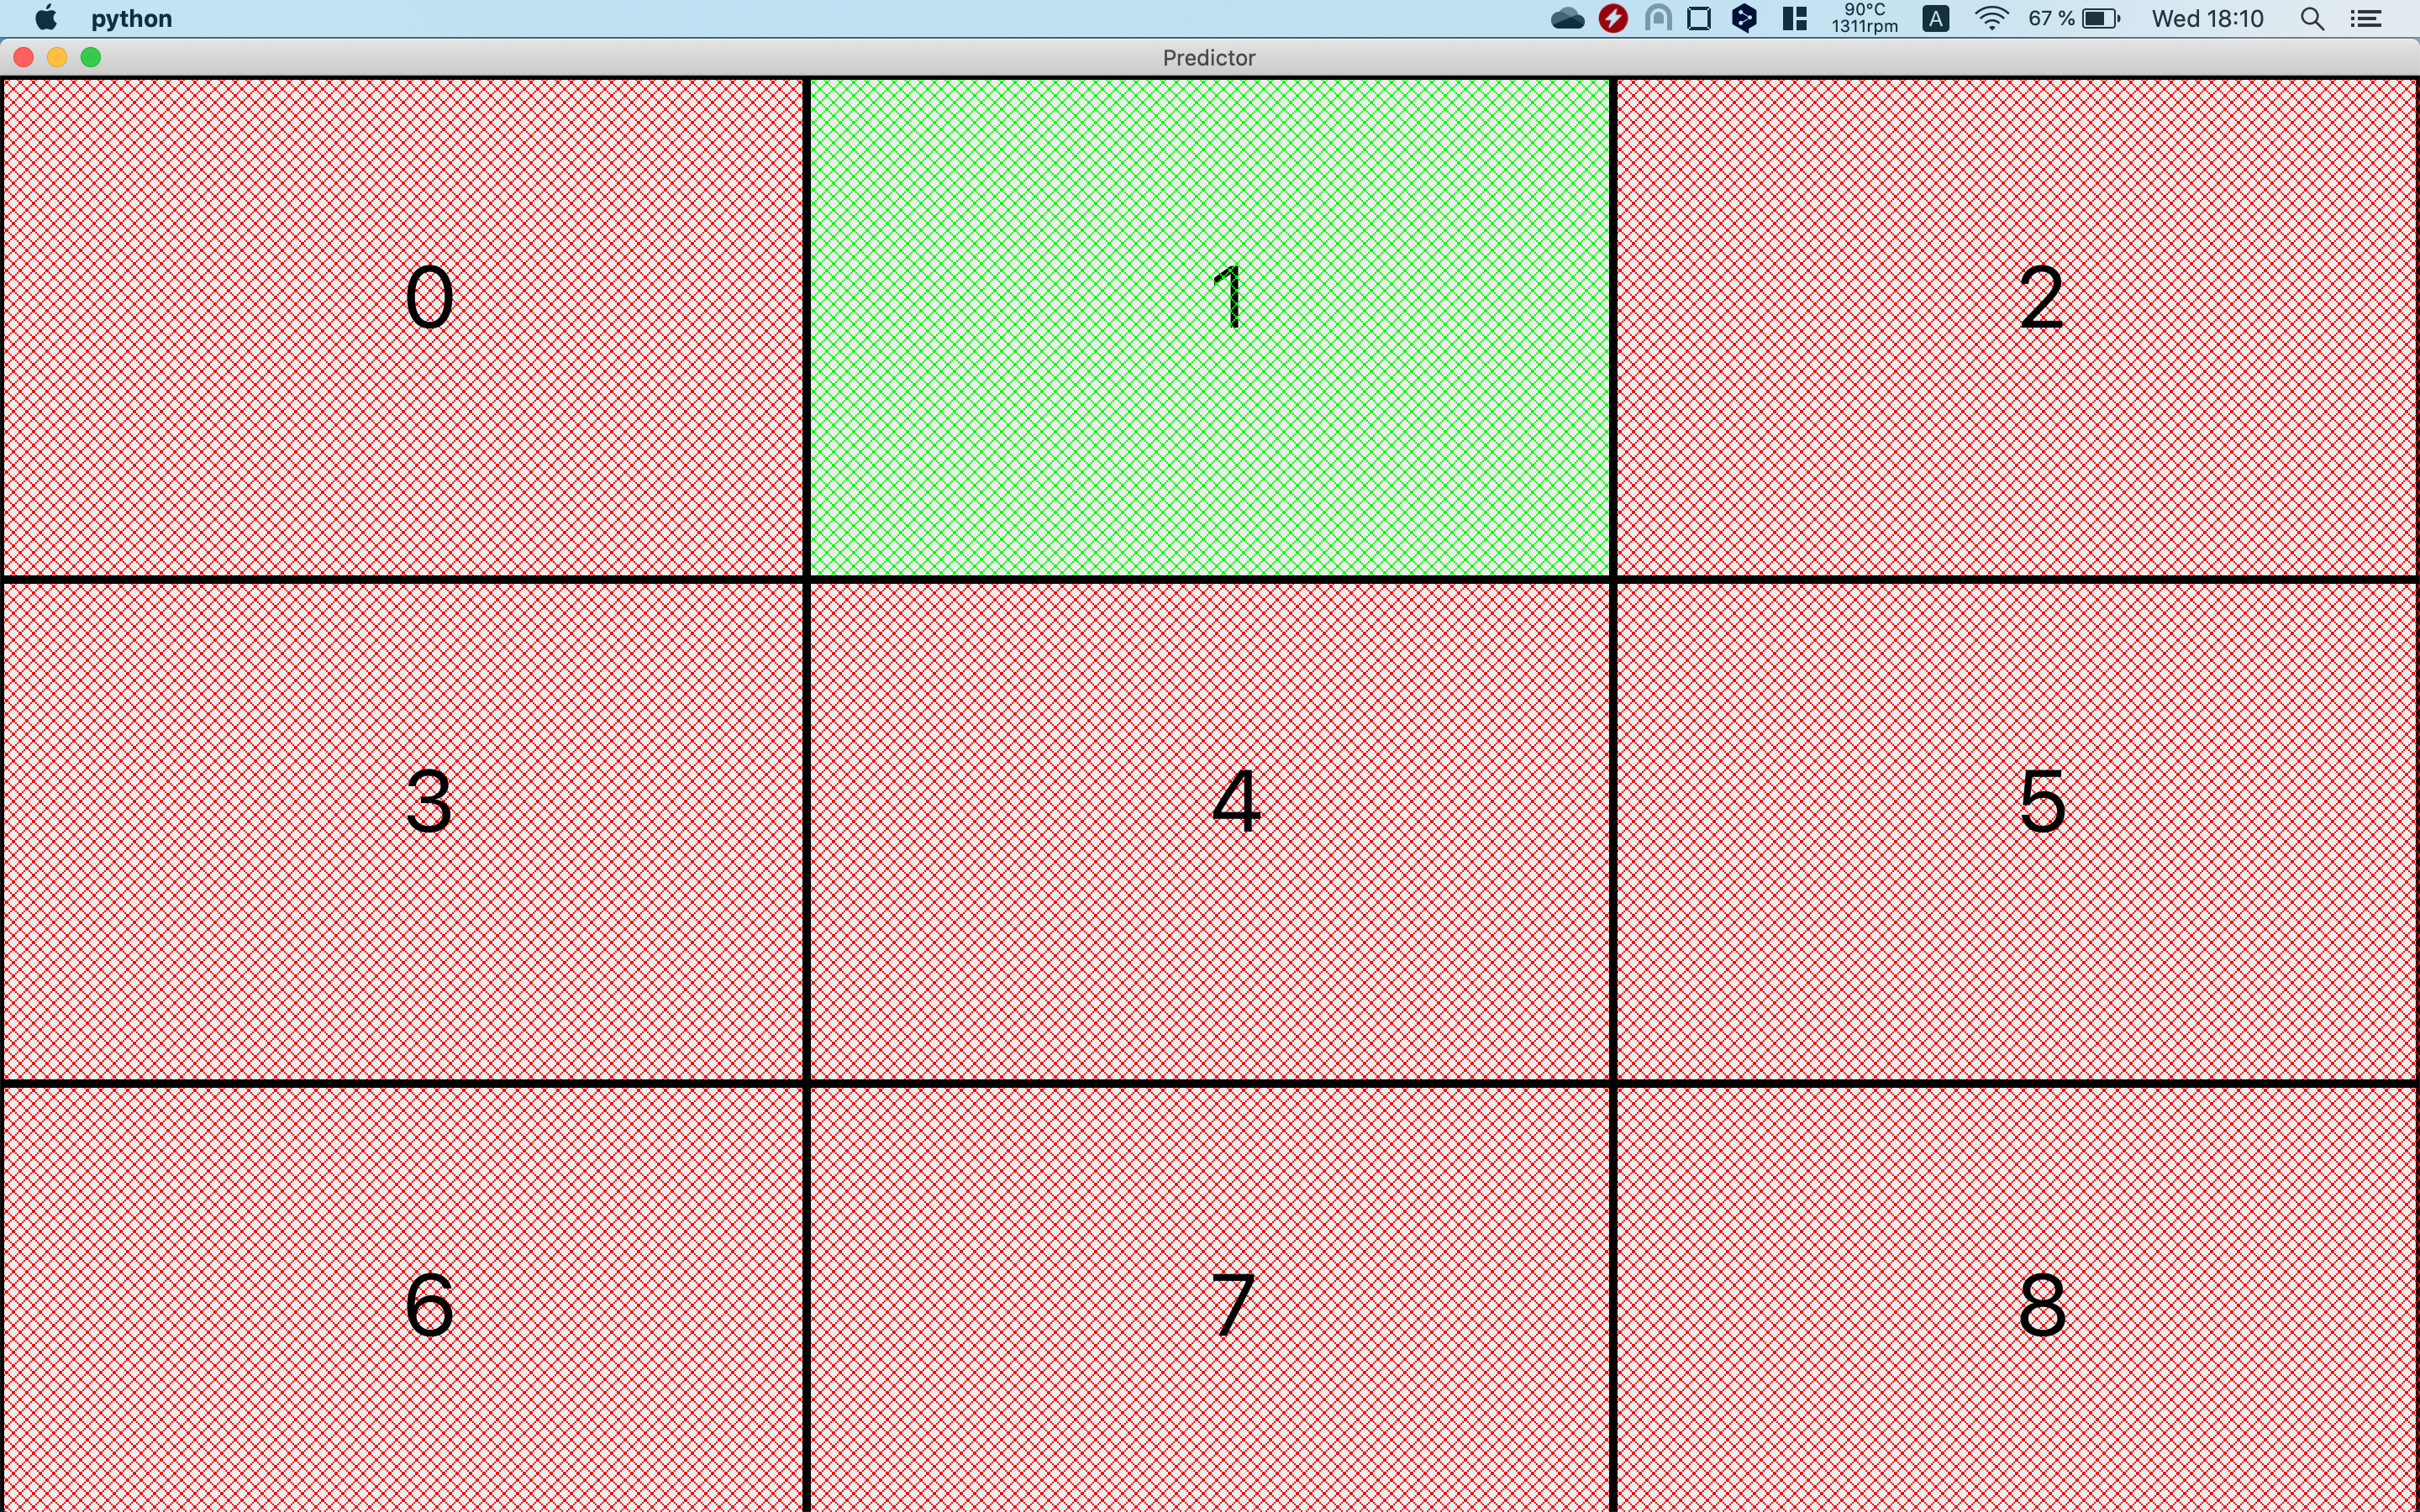
\includegraphics[width=\textwidth/2 - 10pt]{pred1.png}
    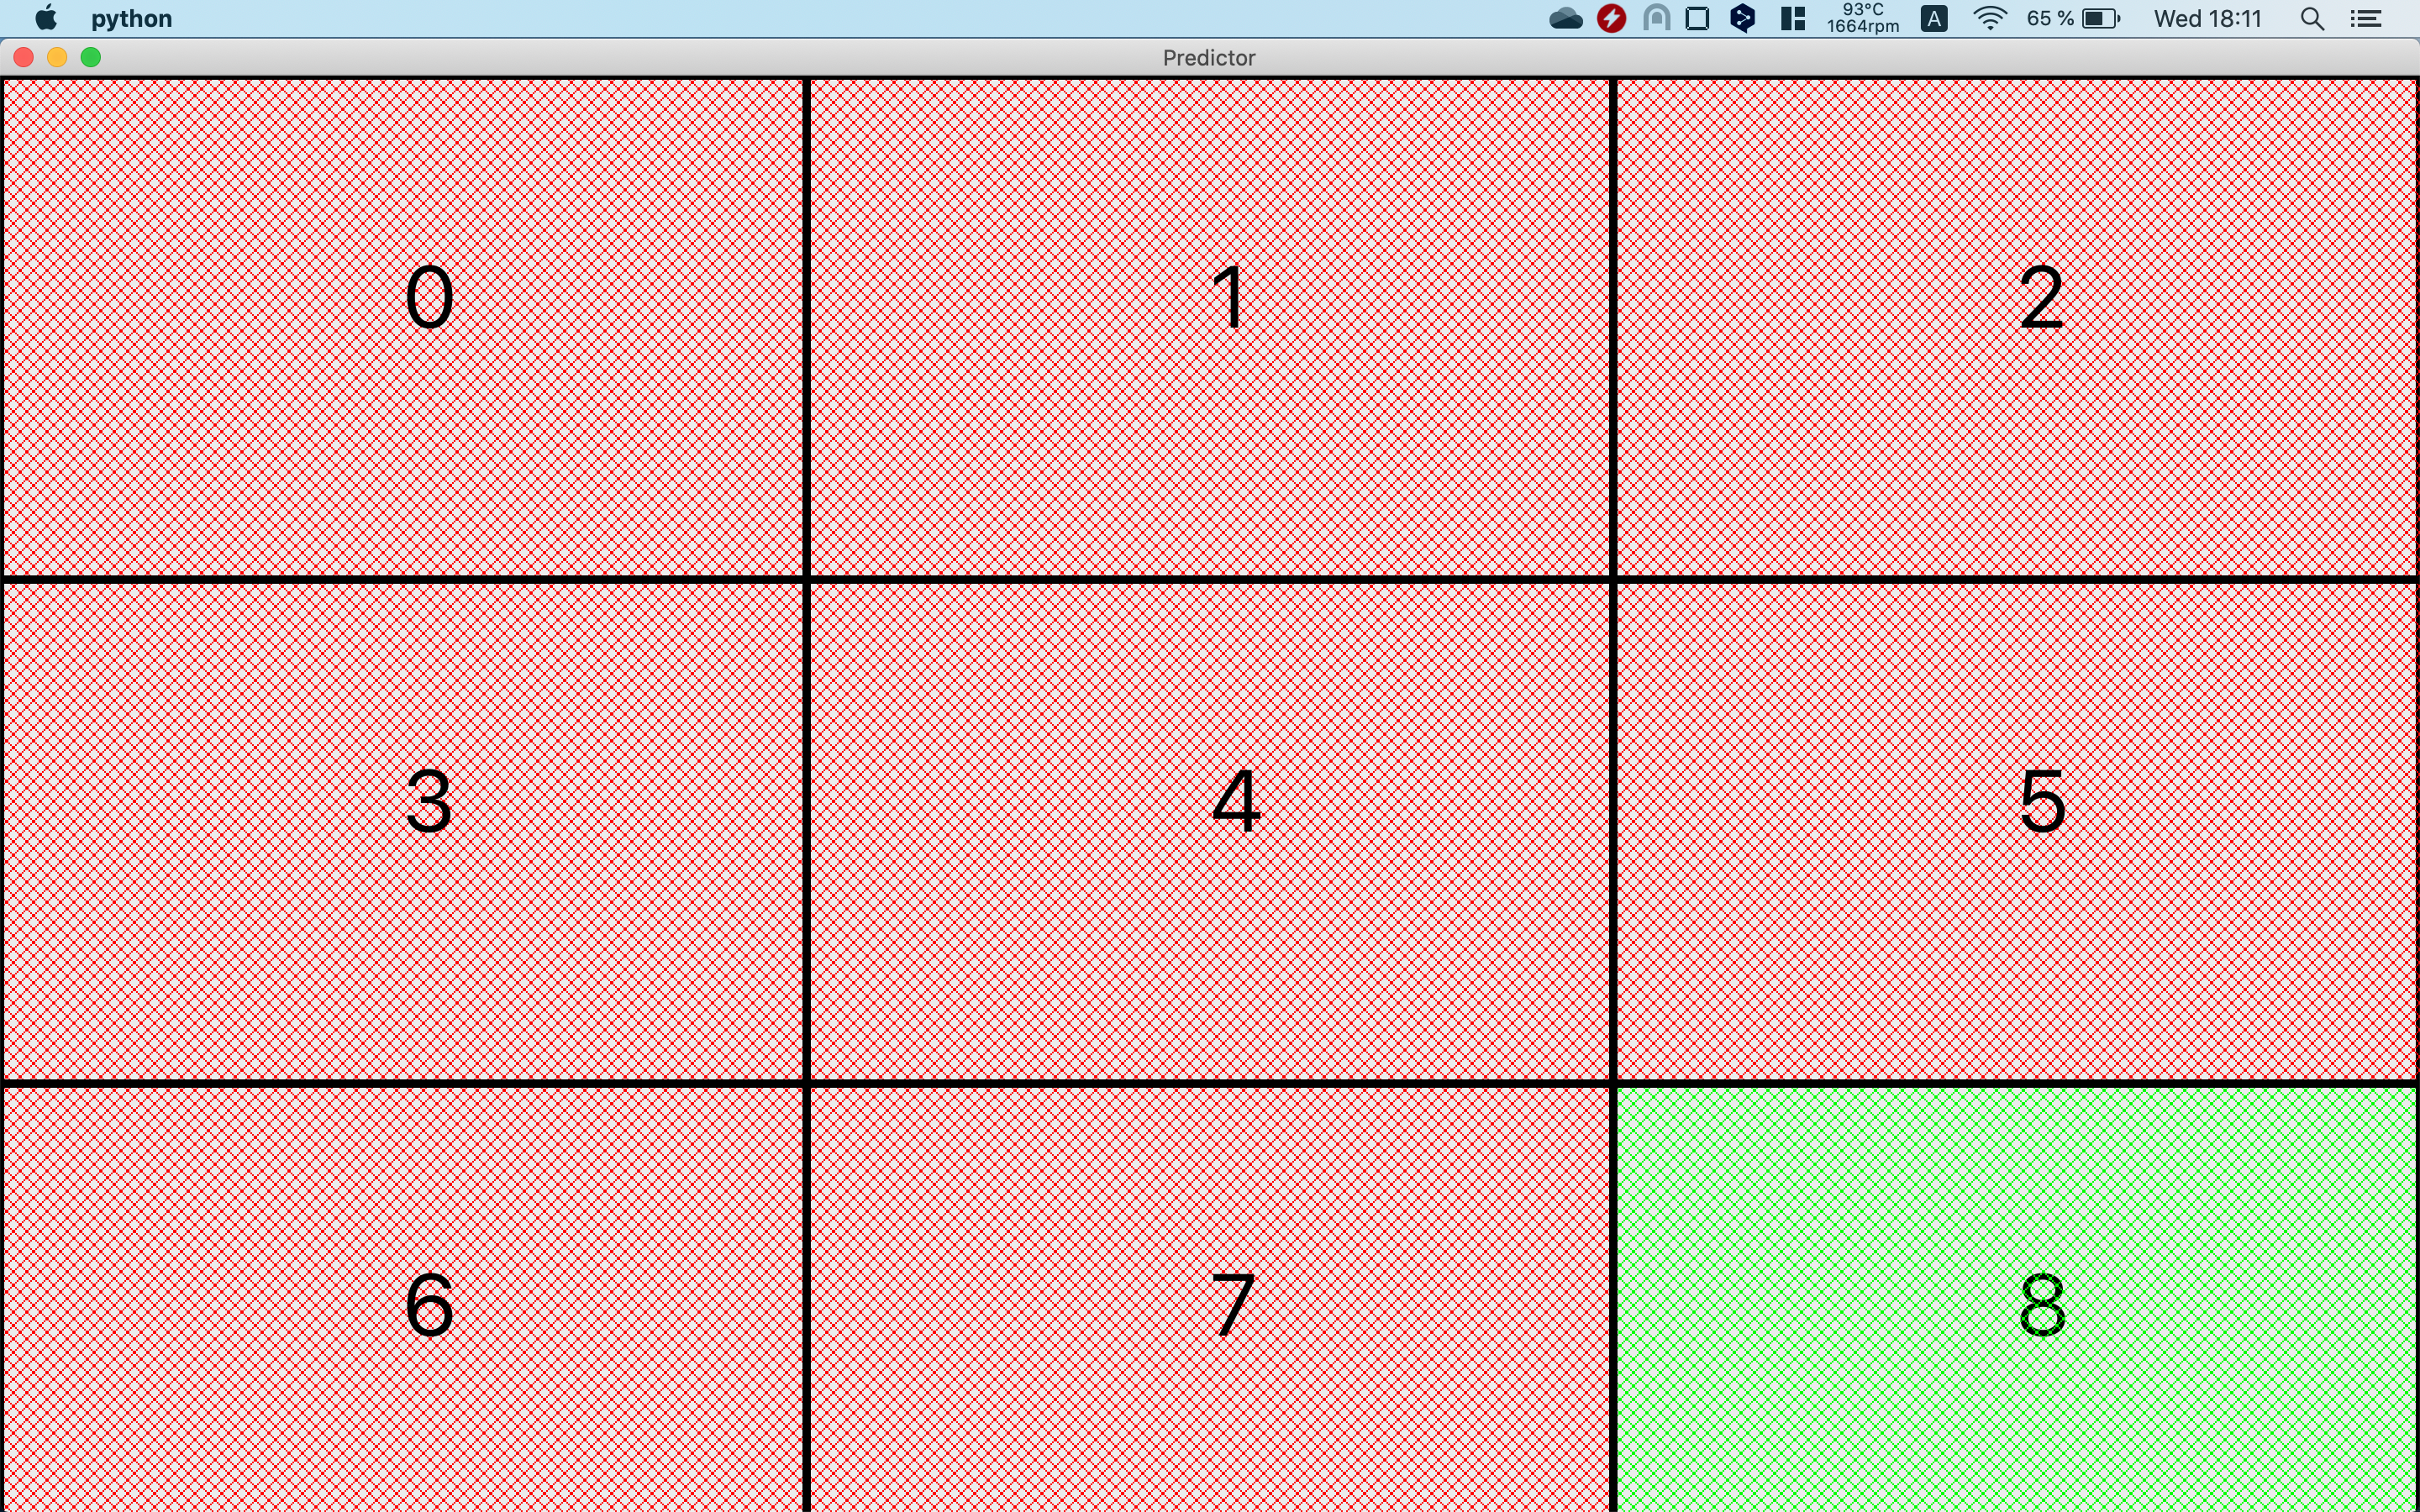
\includegraphics[width=\textwidth/2 - 10pt]{pred2.png}
    \caption{Utiliser les CNN pour suivre les yeux}
\end{figure}

\paragraph{}
Selon \cite{paper_stacked_hourglass}, la méthode ``state-of-the-art'' pour détecter les points de repère faciaux consiste en une architecture ``Hourglass'', qui est, dans sa forme la plus simple, une architecture Encoder–Decoder.

\begin{figure}[h]
    \centering
    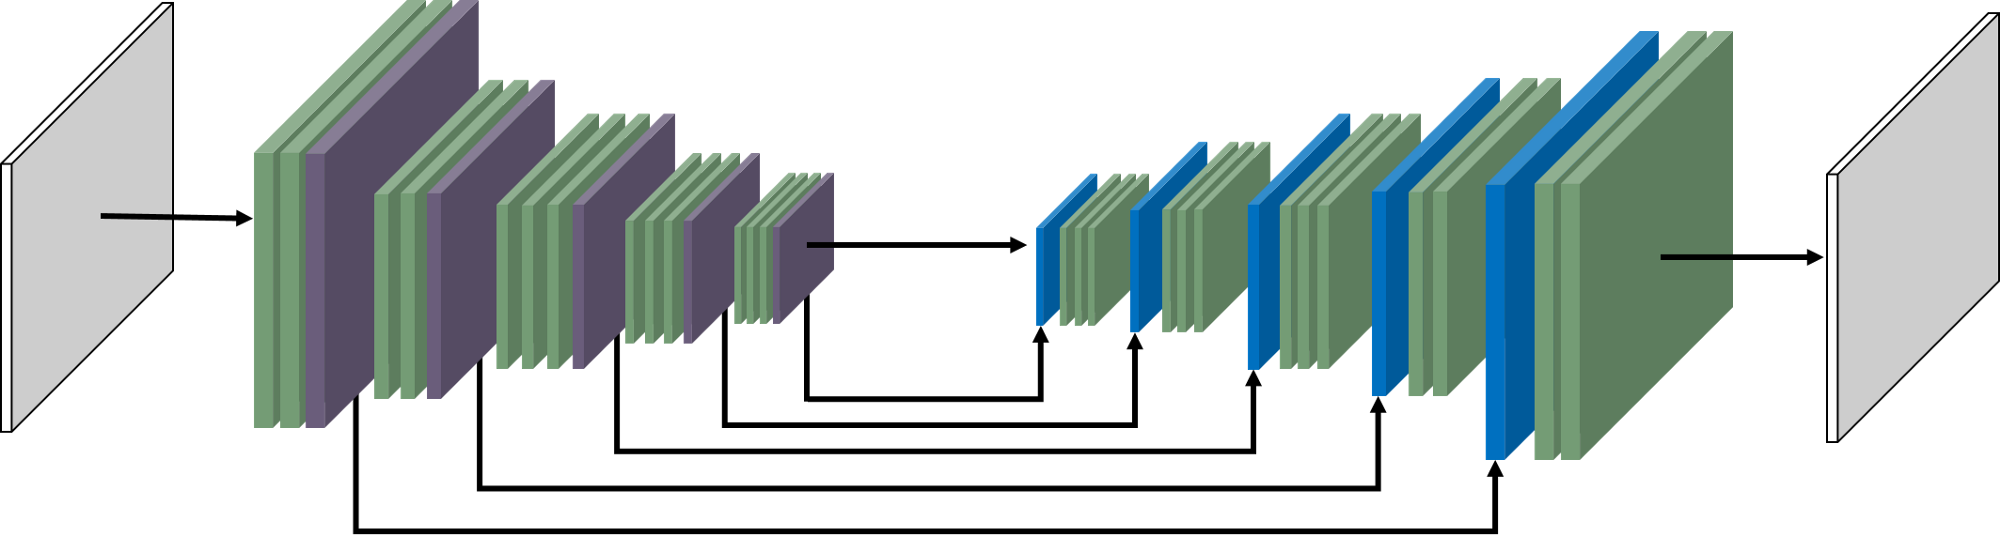
\includegraphics[width=\textwidth]{hourglass.png}
    \caption{Exemple d'architecture Hourglass}
\end{figure}

\paragraph{}
J'ai essayé de ne prédire que le centre de l'oeil à partir d'une image de l'oeil.
Pour obtenir des données de formation, j'ai utilisé le jeu de données de \href{http://cs.uef.fi/pupoint/}{crowdpupil}, qui consiste en $792$ images, chaque image étant étiquetée avec la position du centre de l'oeil.
Il existe deux méthodes pour essayer de prédire les points de repère du visage : essayer de trouver les coordonnées exactes $(x, y)$ par régression, ou essayer de reconstruire des cartes thermiques qui contiennent ces points de repère du visage.

\paragraph{}
J'ai choisi la deuxième option, et j'ai donc généré une carte thermique pour chaque image de l'oeil qui codait le centre de l'oeil.
J'ai mesuré une moyenne pour la distance entre le centre de la pupille et sa marge, et je l'ai utilisée comme ``variance'' pour une Distribution Gaussienne 2D, centrée dans l'oeil.

\begin{figure}[H]
    \centering
    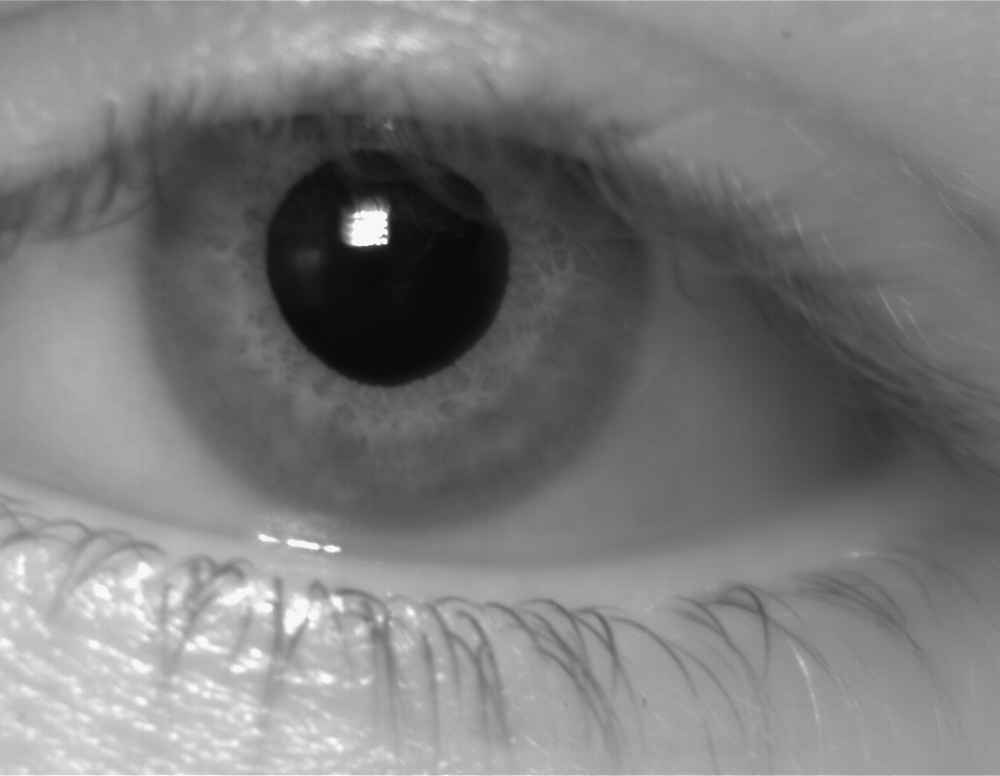
\includegraphics[width=\textwidth/3 - 10pt]{Img_002_L_2.jpg}
    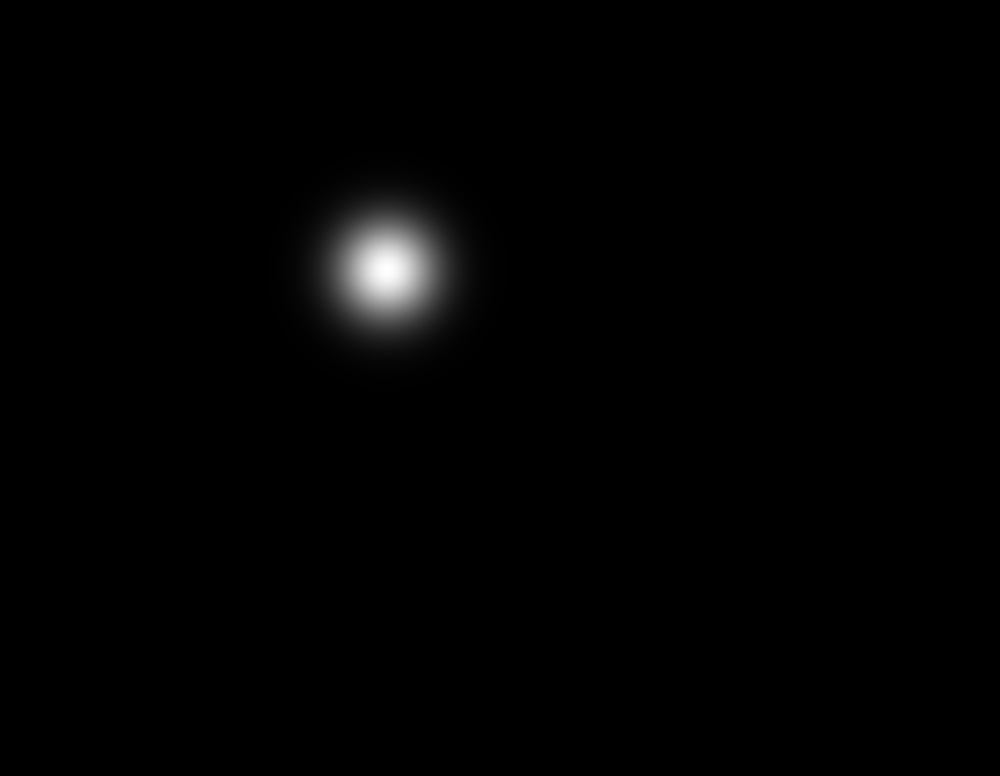
\includegraphics[width=\textwidth/3 - 10pt]{h_Img_002_L_2.jpg}
    \caption{Le centre de l'oeil encodé par un carte thermique}
\end{figure}

\clearpage

\paragraph{}
Après diverses expériences, j'ai découvert que je pouvais assez bien reconstruire les cartes thermiques en utilisant une \emph{architecture simplifiée} de CNN Hourglass :

\begin{lstlisting}[language=python]
class MyCNN(nn.Module):
    def __init__(self, input_size):
        super(MyCNN, self).__init__()
        ## eye image -> encoder -> decoder -> heatmap
        filters = [16, 32, 64, 128]
        # starting encoding
        self.layer1 = nn.Sequential(
            nn.Conv2d(1, filters[0], kernel_size=3, padding=2),
            nn.MaxPool2d(kernel_size=2, stride=2, padding=1),
            nn.ReLU(inplace=True),
            nn.BatchNorm2d(filters[0]),
            
            nn.Conv2d(filters[0], filters[1], kernel_size=2, padding=2),
            nn.MaxPool2d(kernel_size=2, stride=2, padding=1),
            nn.ReLU(inplace=True),
            nn.BatchNorm2d(filters[1]),
            
            nn.Conv2d(filters[1], filters[2], kernel_size=3, padding=2),
            nn.MaxPool2d(kernel_size=2, stride=2, padding=1),
            nn.ReLU(inplace=True),
            nn.BatchNorm2d(filters[2]),
            
            nn.Conv2d(filters[2], filters[3], kernel_size=2, padding=1),
            nn.MaxPool2d(kernel_size=2, stride=2, padding=1),
            nn.ReLU(inplace=True),
            nn.BatchNorm2d(filters[3]),
        )
        # encoding done, starting decoding
        self.layer2 = nn.Sequential(
            nn.Upsample(size=(28, 35), mode='bilinear'),
            nn.ConvTranspose2d(filters[3], filters[2], kernel_size=2, stride=1, padding=1),
            nn.ReLU(inplace=True),
            nn.BatchNorm2d(filters[2]),
            
            nn.Upsample(size=(54, 68), mode='bilinear'),
            nn.ConvTranspose2d(filters[2], filters[1], kernel_size=3, stride=1, padding=2),
            nn.ReLU(inplace=True),
            nn.BatchNorm2d(filters[1]),
            
            nn.Upsample(size=(104, 132), mode='bilinear'),
            nn.ConvTranspose2d(filters[1], filters[0], kernel_size=2, stride=1, padding=2),
            nn.ReLU(inplace=True),
            nn.BatchNorm2d(filters[0]),
        
            nn.Upsample(size=(202, 258), mode='bilinear'),
            nn.ConvTranspose2d(filters[0], 1, kernel_size=3, stride=1, padding=2),
            nn.ReLU(inplace=True),
            nn.BatchNorm2d(1),
        )
\end{lstlisting}

\paragraph{}
J'ai formé le réseau pendant $12$ époques, en utilisant comme optimiseur Adam et comme score MSE.
Pour la dernière époque, la moyenne des erreurs sur l'ensemble des données de test (environ $20\%$ du total des données) était de $8,425983$.
Voici le réseau essayant de reconstruire les cartes thermiques à partir des images des yeux :

\begin{figure}[H]
    \centering
    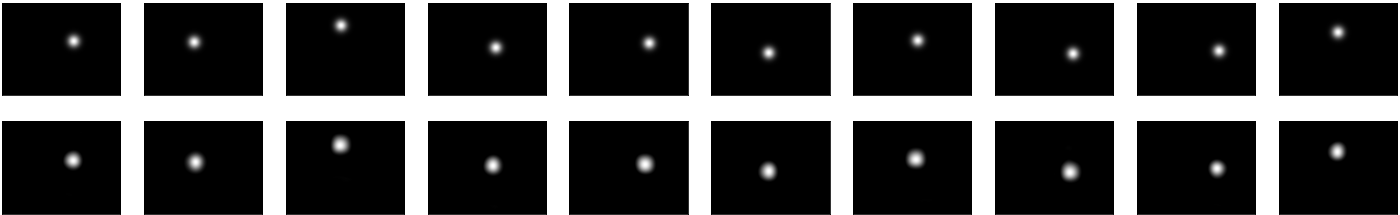
\includegraphics[width=\textwidth - 5pt]{heatmap_predictions.png}
    \caption{Reconstruire les cartes thermiques. La première ligne est le ``ground truth'', la deuxième ligne les prédictions}
\end{figure}

\paragraph{}
Cependant, l'utilisation du réseau sur des images de mes propres yeux n'a pas vraiment donné de bons résultats.
L'une des raisons est que la qualité de ma webcam n'est pas très bonne et que les images des yeux extraites étaient très bruyantes.
% However, using the network on images of my own eyes didn't really give good results.
% One of the reasons is that my webcam's quality isn't very good and the images of the extracted eyes were very noisy.

\begin{figure}[H]
    \centering
    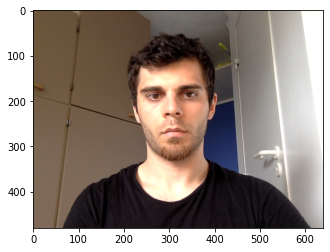
\includegraphics[width=\textwidth/3 - 5pt]{heatmap_test.png}
    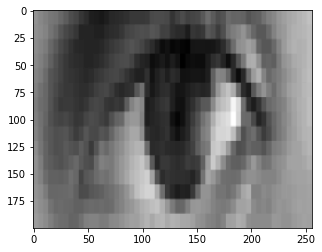
\includegraphics[width=\textwidth/3 - 5pt]{heatmap_eye.png}
    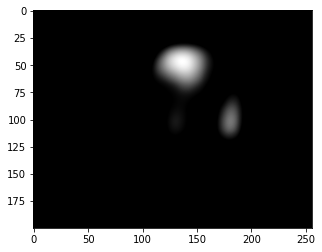
\includegraphics[width=\textwidth/3 - 5pt]{heatmap_result.png}
    \caption{Tester le réseau Hourglass sur des images de moi-même}
\end{figure}




% After successfully using the CNN architecture to predict the area where the user is looking, I became interested in how the facial landmarks can be detected.
% =======insert img with prediction========
% According to [], the current "state-of-the-art" method for detecting facial landmarks consists in an Hourglass Architecture, which is, in its simplest form, an Encoder-Decoder architecture.

% I tried to predict only the center of the eye from an eye image. To get training data, I used crowdpupil's dataset, which consists of 792 images, each image being labeled with the position of the center of the eye.
% There are 2 methods in trying to predict facial landmarks: try to find the exact coordinates (x, y) through regression, or try to reconstruct heatmaps that contain those facial landmarks.
% I went with the second option, so I generated a heatmap for each eye image that encoded the center of the eye.
% I measured an average for the distance between the center of the pupil and its margin, and I used that as the variange for a 2D Gaussian Distribution, centered in the eye.

%==========insert eye with heatmap================

% After various experiments, I found that I can reconstruct the heatmaps fairly well using this CNN Hourglass architecture:
% insert code

% Here are the results:

